\documentclass[tikz, border=1mm]{standalone}
\begin{document}
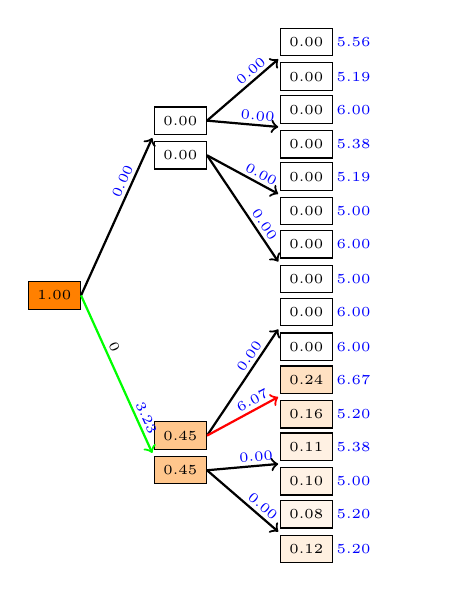
\begin{tikzpicture}
\tikzstyle{between} = [rectangle, minimum height=0.10cm, minimum width=0.70cm, draw opacity=0]
\tikzstyle{qval}    = [rectangle, text centered, text width=2cm]
\node[between] at (-8.40, 2.00) (1_b_0){};
\node[between] at (-8.40, -2.00) (1_b_1){};
\node[between] at (-6.80, 3.00) (2_b_0){};
\node[between] at (-6.80, 2.14) (2_b_1){};
\node[between] at (-6.80, 1.29) (2_b_2){};
\node[between] at (-6.80, 0.43) (2_b_3){};
\node[between] at (-6.80, -0.43) (2_b_4){};
\node[between] at (-6.80, -1.29) (2_b_5){};
\node[between] at (-6.80, -2.14) (2_b_6){};
\node[between] at (-6.80, -3.00) (2_b_7){};
\node[rectangle, text centered, draw=black, minimum height=0.20cm, minimum width=0.45cm, fill=orange, fill opacity=1.00, draw opacity=1, text opacity=1] at (-10.00, 0.00) (0_s_0) {\tiny 1.00};
\node[rectangle, text centered, draw=black, minimum height=0.20cm, minimum width=0.45cm, fill=orange, fill opacity=0.00, draw opacity=1, text opacity=1] at (-8.40, 2.22) (1_s_0) {\tiny 0.00};
\node[rectangle, text centered, draw=black, minimum height=0.20cm, minimum width=0.45cm, fill=orange, fill opacity=0.00, draw opacity=1, text opacity=1] at (-8.40, 1.78) (1_s_1) {\tiny 0.00};
\node[rectangle, text centered, draw=black, minimum height=0.20cm, minimum width=0.45cm, fill=orange, fill opacity=0.45, draw opacity=1, text opacity=1] at (-8.40, -1.78) (1_s_2) {\tiny 0.45};
\node[rectangle, text centered, draw=black, minimum height=0.20cm, minimum width=0.45cm, fill=orange, fill opacity=0.45, draw opacity=1, text opacity=1] at (-8.40, -2.22) (1_s_3) {\tiny 0.45};
\node[rectangle, text centered, draw=black, minimum height=0.20cm, minimum width=0.45cm, fill=orange, fill opacity=0.00, draw opacity=1, text opacity=1] at (-6.80, 3.22) (2_s_0) {\tiny 0.00};
\node[qval] at (-6.20, 3.22) () {\tiny \textcolor{blue}{5.56}};
\node[rectangle, text centered, draw=black, minimum height=0.20cm, minimum width=0.45cm, fill=orange, fill opacity=0.00, draw opacity=1, text opacity=1] at (-6.80, 2.78) (2_s_1) {\tiny 0.00};
\node[qval] at (-6.20, 2.78) () {\tiny \textcolor{blue}{5.19}};
\node[rectangle, text centered, draw=black, minimum height=0.20cm, minimum width=0.45cm, fill=orange, fill opacity=0.00, draw opacity=1, text opacity=1] at (-6.80, 2.36) (2_s_2) {\tiny 0.00};
\node[qval] at (-6.20, 2.36) () {\tiny \textcolor{blue}{6.00}};
\node[rectangle, text centered, draw=black, minimum height=0.20cm, minimum width=0.45cm, fill=orange, fill opacity=0.00, draw opacity=1, text opacity=1] at (-6.80, 1.92) (2_s_3) {\tiny 0.00};
\node[qval] at (-6.20, 1.92) () {\tiny \textcolor{blue}{5.38}};
\node[rectangle, text centered, draw=black, minimum height=0.20cm, minimum width=0.45cm, fill=orange, fill opacity=0.00, draw opacity=1, text opacity=1] at (-6.80, 1.51) (2_s_4) {\tiny 0.00};
\node[qval] at (-6.20, 1.51) () {\tiny \textcolor{blue}{5.19}};
\node[rectangle, text centered, draw=black, minimum height=0.20cm, minimum width=0.45cm, fill=orange, fill opacity=0.00, draw opacity=1, text opacity=1] at (-6.80, 1.07) (2_s_5) {\tiny 0.00};
\node[qval] at (-6.20, 1.07) () {\tiny \textcolor{blue}{5.00}};
\node[rectangle, text centered, draw=black, minimum height=0.20cm, minimum width=0.45cm, fill=orange, fill opacity=0.00, draw opacity=1, text opacity=1] at (-6.80, 0.65) (2_s_6) {\tiny 0.00};
\node[qval] at (-6.20, 0.65) () {\tiny \textcolor{blue}{6.00}};
\node[rectangle, text centered, draw=black, minimum height=0.20cm, minimum width=0.45cm, fill=orange, fill opacity=0.00, draw opacity=1, text opacity=1] at (-6.80, 0.21) (2_s_7) {\tiny 0.00};
\node[qval] at (-6.20, 0.21) () {\tiny \textcolor{blue}{5.00}};
\node[rectangle, text centered, draw=black, minimum height=0.20cm, minimum width=0.45cm, fill=orange, fill opacity=0.00, draw opacity=1, text opacity=1] at (-6.80, -0.21) (2_s_8) {\tiny 0.00};
\node[qval] at (-6.20, -0.21) () {\tiny \textcolor{blue}{6.00}};
\node[rectangle, text centered, draw=black, minimum height=0.20cm, minimum width=0.45cm, fill=orange, fill opacity=0.00, draw opacity=1, text opacity=1] at (-6.80, -0.65) (2_s_9) {\tiny 0.00};
\node[qval] at (-6.20, -0.65) () {\tiny \textcolor{blue}{6.00}};
\node[rectangle, text centered, draw=black, minimum height=0.20cm, minimum width=0.45cm, fill=orange, fill opacity=0.24, draw opacity=1, text opacity=1] at (-6.80, -1.07) (2_s_10) {\tiny 0.24};
\node[qval] at (-6.20, -1.07) () {\tiny \textcolor{blue}{6.67}};
\node[rectangle, text centered, draw=black, minimum height=0.20cm, minimum width=0.45cm, fill=orange, fill opacity=0.16, draw opacity=1, text opacity=1] at (-6.80, -1.51) (2_s_11) {\tiny 0.16};
\node[qval] at (-6.20, -1.51) () {\tiny \textcolor{blue}{5.20}};
\node[rectangle, text centered, draw=black, minimum height=0.20cm, minimum width=0.45cm, fill=orange, fill opacity=0.11, draw opacity=1, text opacity=1] at (-6.80, -1.92) (2_s_12) {\tiny 0.11};
\node[qval] at (-6.20, -1.92) () {\tiny \textcolor{blue}{5.38}};
\node[rectangle, text centered, draw=black, minimum height=0.20cm, minimum width=0.45cm, fill=orange, fill opacity=0.10, draw opacity=1, text opacity=1] at (-6.80, -2.36) (2_s_13) {\tiny 0.10};
\node[qval] at (-6.20, -2.36) () {\tiny \textcolor{blue}{5.00}};
\node[rectangle, text centered, draw=black, minimum height=0.20cm, minimum width=0.45cm, fill=orange, fill opacity=0.08, draw opacity=1, text opacity=1] at (-6.80, -2.78) (2_s_14) {\tiny 0.08};
\node[qval] at (-6.20, -2.78) () {\tiny \textcolor{blue}{5.20}};
\node[rectangle, text centered, draw=black, minimum height=0.20cm, minimum width=0.45cm, fill=orange, fill opacity=0.12, draw opacity=1, text opacity=1] at (-6.80, -3.22) (2_s_15) {\tiny 0.12};
\node[qval] at (-6.20, -3.22) () {\tiny \textcolor{blue}{5.20}};
\draw[->, thick, black] (0_s_0.east) -- (1_b_0.west) node [pos=0.70, above=-0.2em, sloped, font=\tiny] () {\textcolor{blue}{0.00}};
\draw[->, thick, green] (0_s_0.east) -- (1_b_1.west) node [pos=0.35, above=-0.2em, sloped, font=\tiny] () {\textcolor{black}{0}} node [pos=0.80, above=-0.2em, sloped, font=\tiny] () {\textcolor{blue}{3.23}};
\draw[->, thick, black] (1_s_0.east) -- (2_b_0.west) node [pos=0.70, above=-0.2em, sloped, font=\tiny] () {\textcolor{blue}{0.00}};
\draw[->, thick, black] (1_s_0.east) -- (2_b_1.west) node [pos=0.70, above=-0.2em, sloped, font=\tiny] () {\textcolor{blue}{0.00}};
\draw[->, thick, black] (1_s_1.east) -- (2_b_2.west) node [pos=0.70, above=-0.2em, sloped, font=\tiny] () {\textcolor{blue}{0.00}};
\draw[->, thick, black] (1_s_1.east) -- (2_b_3.west) node [pos=0.70, above=-0.2em, sloped, font=\tiny] () {\textcolor{blue}{0.00}};
\draw[->, thick, black] (1_s_2.east) -- (2_b_4.west) node [pos=0.70, above=-0.2em, sloped, font=\tiny] () {\textcolor{blue}{0.00}};
\draw[->, thick, red] (1_s_2.east) -- (2_b_5.west) node [pos=0.70, above=-0.2em, sloped, font=\tiny] () {\textcolor{blue}{6.07}};
\draw[->, thick, black] (1_s_3.east) -- (2_b_6.west) node [pos=0.70, above=-0.2em, sloped, font=\tiny] () {\textcolor{blue}{0.00}};
\draw[->, thick, black] (1_s_3.east) -- (2_b_7.west) node [pos=0.70, above=-0.2em, sloped, font=\tiny] () {\textcolor{blue}{0.00}};
\end{tikzpicture}
\end{document}